\documentclass[a4paper,12pt]{article}
\usepackage[utf8]{inputenc}
\usepackage[english,greek]{babel}
\usepackage{lmodern} 
\usepackage{hyperref}
\usepackage{subcaption}
\usepackage{graphicx}
\usepackage{amsmath}
\usepackage{float}

\title{Υλοποίηση εξελικτικού πρωταθλήματος \foreignlanguage{english}{Axelrod}}
\author{Γιώργος Γκιουλέκας \\ Ελένη Κουμπαρίδου \\ Ναταλία-Αναστασία Κούστα}
\date{Απρίλιος 2025}

\begin{document}
\maketitle
\tableofcontents

\section{Εισαγωγή}
Στην παρούσα αναφορά, αναλύουμε την υλοποίηση του εξελικτικού πρωταθλήματος \foreignlanguage{english}{Axelrod}, χρησιμοποιώντας τις έννοιες των \foreignlanguage{english}{Fitness} και \foreignlanguage{english}{Imitation Dynamics.} Έχουμε υλοποιήσει 9 διαφορετικές στρατηγικές, ο κώδικας των οποίων μπορεί να βρεθεί στον φάκελο \foreignlanguage{english}{Strategies} του \foreignlanguage{english}{project}. Το μόνο που χρειάζεται να κάνει κάποιος είναι να ανοίξει το αρχείο  \foreignlanguage{english}{main.m} και από εκεί μπορεί να τρέξει το κάθε \foreignlanguage{english}{section} ξεχωριστά για κάθε μία από τις 4 ζητούμενες συναρτήσεις. Οι παράμετροι που ορίζονται στην αρχή εφαρμόζονται σε όλες τις ακόλουθες συναρτήσεις εκτός από την \foreignlanguage{english}{TourTheImi} όπου ορίζουμε διαφορετικούς πληθυσμούς, λόγω της εκθετικής ανάγκης σε μνήμη.


\section{Εξελικτικό πρωτάθλημα με \foreignlanguage{english}{Fitness Dynamics}}
Η υλοποίηση του εξελικτικού πρωταθλήματος με τη χρήση των \foreignlanguage{english}{Fitness Dynamics} βασίστηκε στο \foreignlanguage{english}{paper} \foreignlanguage{english}{"Studies on Dynamics in the Classical Iterated Prisoner’s Dilemma with Few Strategies"}.

\subsection{Προσομοίωση πρωταθλήματος \foreignlanguage{english}{- TourSimFit}}


\subsubsection*{Υπολογισμός \foreignlanguage{english}{Fitness}}
Σε κάθε γενεά, υπολογίζουμε την τιμή \foreignlanguage{english}{Fitness} για κάθε στρατηγική με βάση τους πόντους που έχουν συγκεντρώσει οι παίκτες της συγκεκριμένης στρατηγικής συνολικά κατά τη διάρκεια του πρωταθλήματος. Η στρατηγική με την υψηλότερη τιμή \foreignlanguage{english}{Fitness} θεωρείται η καλύτερη.


\subsubsection*{Ανακατανομή πληθυσμού}
Για την ανακατανομή του πληθυσμού, χρησιμοποιούμε τη συνάρτηση \foreignlanguage{english}{pop\_redistribute}. Αρχικά, υπολογίζουμε την ισχύ κάθε στρατηγικής, η οποία είναι η συνολική βαθμολογία των παικτών της διαιρεμένη με τους συνολικούς πόντους του πρωταθλήματος. Αυτή η αναλογία πολλαπλασιάζεται με το συνολικό πληθυσμό για να προσδιοριστεί το αναλογικό πλήθος παικτών για κάθε στρατηγική. Στη συνέχεια, το αποτέλεσμα στρογγυλοποιείται προς τα κάτω για κάθε στρατηγική. Τέλος, οι παίκτες που περισσεύουν κατανέμονται στις στρατηγικές με τις μεγαλύτερες απώλειες λόγω της στρογγυλοποίησης.



\subsection{Θεωρητική ανάλυση πρωταθλήματος \foreignlanguage{english}{-TourTheFit}}
Η θεωρητική ανάλυση του πρωταθλήματος βασίζεται ακριβώς στην ανάλυση που περιγράφεται στο \foreignlanguage{english}{paper} που αναφέρθηκε προηγουμένως. Στην ανάλυση αυτή, ο υπολογισμός της \foreignlanguage{english}{Fitness} πραγματοποιείται με βάση τον πίνακα απολαβών ενός παίκτη μιας στρατηγικής με έναν παίκτη μιας άλλης. Ο πίνακας έχει προσδιοριστεί θεωρητικά για 1000 γύρους/\foreignlanguage{english}{match} όπως και στο \foreignlanguage{english}{paper} (αποθηκευμένος στο αρχείο \foreignlanguage{english}{excel V\_{matrix})}. Για διαφορετικό αριθμό γύρων ο πίνακας προσδιορίζεται με προσομοίωση μέσω της συνάρτησης \foreignlanguage{english}{ComputePayoffMatrix}. Στη συνέχεια ακολουθούμε τα παρακάτω βήματα για την ανακατανομή του πληθυσμού στην επόμενη γενεά:

\begin{enumerate}

\item \textbf{Συνολικός πληθυσμός ανά γενιά:} Άθροισμα των αριθμών παικτών της κάθε στρατηγικής:
\begin{equation}
P = \sum_{i=1}^S W_n(i)
\end{equation}

\item \textbf{Σκορ παίκτη κάθε στρατηγικής \(g(i)\):} Για τον υπολογισμό του σκορ ενός παίκτη κάθε στρατηγικής, αθροίζουμε τους παίκτες κάθε στρατηγικής με το κέρδος του παίκτη για κάθε παιχνίδι με αυτήν την στρατηγική. Αφαιρούμε μία φορά το κέρδος με αντίπαλο ίδιας στρατηγικής αφού ο παίκτης δεν παίζει με τον εαυτό του: 
\begin{equation}
g_n(i) = \sum_{j=1}^{S} W_n(j) \cdot V(i, j) - V(i, i)
\end{equation}

\item \textbf{Συνολικοί πόντοι του πρωταθλήματος:} Υπολογίζουμε τους συνολικούς πόντους του πρωταθλήματος αθροίζοντας για κάθε στρατηγική, το γινόμενο του πλήθους των παικτών αυτής με τους πόντους που συνέλεξε καθένας από τους παίκτες της:
\begin{equation}
\text{\foreignlanguage{english}{TotalPoints}} = \sum_{i=1}^S W_n(i) \cdot g_n(i)
\end{equation}

\item \textbf{Ανακατανομή πληθυσμού της επόμενης γενεάς:} Υπολογισμός του αριθμού των παικτών κάθε στρατηγικής στην επόμενη γενεά με εκπροσώπηση ανάλογη του ποσοστού των συνολικών πόντων μιας στρατηγικής επί των συνολικών πόντων του πρωταθλήματος
\begin{equation}
W_{n+1}(i) = P \cdot \frac{W_n(i) \cdot g_n(i)}{\text{\foreignlanguage{english}{TotalPoints}}}
\end{equation}

\end{enumerate}

\subsection{Πειράματα}
\subsubsection*{Πρωτάθλημα μεταξύ των στρατηγικών \foreignlanguage{english}{(CD)*, (DDC)*, Soft-Majo}}
Στο πρώτο πείραμα, πραγματοποιήσαμε ένα πρωτάθλημα μεταξύ των στρατηγικών \foreignlanguage{english}{(CD)$^*$, (DDC)$^*$ }και \foreignlanguage{english}{\text{Soft-Majo}}. Αρχικοποιήσαμε τον πληθυσμό με 100 παίκτες για κάθε στρατηγική και ορίσαμε τον πίνακα αποδόσεων ως:
\[
B = \begin{bmatrix}
3 & 0 \\
5 & 1
\end{bmatrix}
\]
Στο Σχήμα 1 παρουσιάζονται η θεωρητική ανάλυση και η προσομοίωση του προαναφερόντος εξελικτικού πρωταθλήματος χρησιμοποιώντας τη μέθοδο \foreignlanguage{english}{Fitness Dynamics}.

Μια παρατήρηση που πρέπει να γίνει έχει να κάνει με τον αριθμό των γύρων σε κάθε \foreignlanguage{english}{match} που ορίσαμε. Επειδή γίνεται προσομοίωση παίκτη-παίκτη για πολλές γενιές, μειώσαμε τον αριθμό των γύρων σε 100 αντί για 1000 που ήταν στην θεωρητική ανάλυση, ώστε να μειώσουμε τον χρόνο της προσομοίωσης που ακόμη και με 100 γύρους ήταν μεγάλος. Παρόλα αυτά τα αποτελέσματα φαίνεται να συμβαδίζουν.

Εντοπίζεται μια ανάκαμψη της \foreignlanguage{english}{Soft-Majo} μετά την γενιά 60 η οποία οφείλεται από την μία στο γεγονός ότι ο πληθυσμός της δεν μηδενίστηκε μεταξύ των γενεών 20-40, απλά σταθεροποιήθηκε περίπου στους 1.5-2 παίκτες (επιτρέπουμε δεκαδικούς παίκτες στην θεωρητική ανάλυση), και εκμεταλλεύτηκε την πτώση του πληθυσμού της \foreignlanguage{english}{(CD)*} για να κερδίσει πληθυσμό για μερικές (περίπου 40) γενιές πριν τον ξαναχάσει.


\begin{figure}[H]
    \centering
    \begin{minipage}{0.5\linewidth}
        \centering
        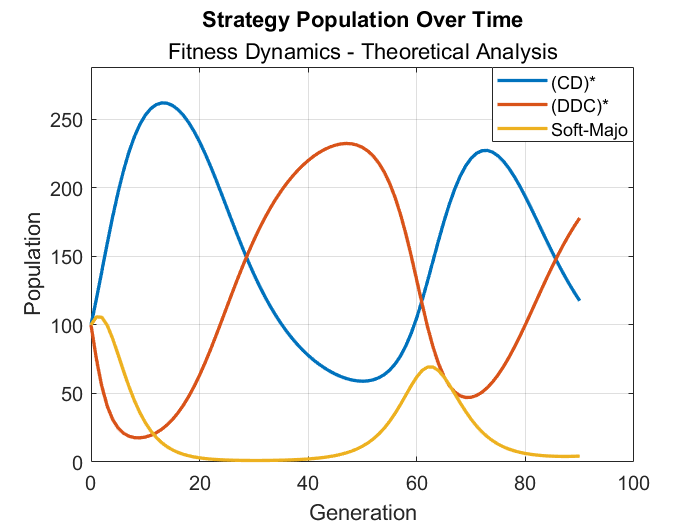
\includegraphics[width=\linewidth]{Graphs/fit_the1a.png}
        \label{fig:fit_the1a}
    \end{minipage}%    
    \begin{minipage}{0.5\linewidth}
        \centering
        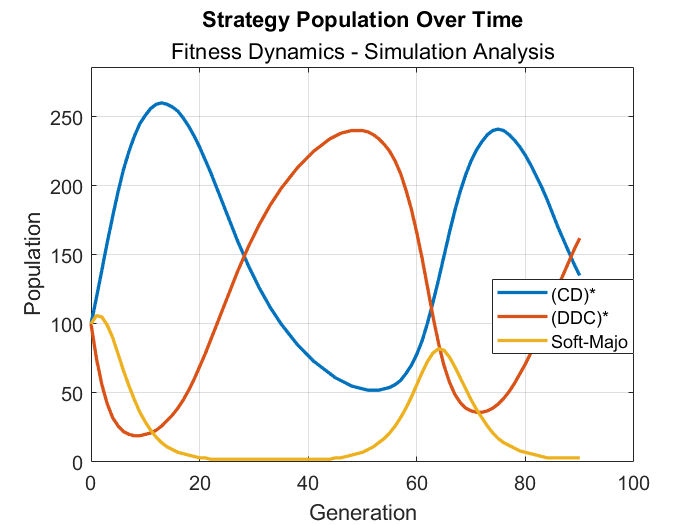
\includegraphics[width=\linewidth]{Graphs/fit_sim1.png}
        \label{fig:fit_sim1}
    \end{minipage}
    \caption{Ανάλυση και Προσομοίωση με \foreignlanguage{english}{Fitness Dynamics}}
\end{figure}



\subsubsection*{Πρωτάθλημα μεταξύ των στρατηγικών \foreignlanguage{english}{(CCD)*, (DDC)*, Soft-Majo}}

Στο δεύτερο πείραμα, πραγματοποιήσαμε ένα πρωτάθλημα μεταξύ των στρατηγικών \foreignlanguage{english}{(CCD)*}, \foreignlanguage{english}{(DDC)*} και \foreignlanguage{english}{\text{Soft-Majo}}. Ο αρχικός αριθμός παικτών ήταν 300, 200 και 100 αντίστοιχα, ενώ διατηρήσαμε τον ίδιο πίνακα απολαβών. Αξίζει να παρατηρήσουμε στα διαγράμματα \ref{fig:the_fit2_dec} και \ref{fig:the_fit2_pr} που ακολουθούν, πως η θεωρητική ανάλυση εμφανίζει διαφορετικά αποτελέσματα ανάλογα με τον τρόπο που κάνουμε την αναπροσαρμογή του πληθυσμού της νέας γενιάς. Εάν επιτρέψουμε δεκαδικούς αριθμούς για πλήθος παικτών τότε έχουμε αποσβεννύμενες ταλαντώσεις (αυτό επειδή επιτρέπουμε το σημείο ισορροπίας των πληθυσμών να βρεθεί σε μη ακέραια τιμή), ενώ αν τους στρογγυλοποιήσουμε σε ακέραιους μέσω της \foreignlanguage{english}{pop\_redistribute} (όπως συμβαίνει και στο \foreignlanguage{english}{paper}) τότε οι ταλαντώσεις διατηρούν το πλάτος τους. Στην προσομοίωση, επειδή κάνουμε στρογγυλοποίηση των πληθυσμών σε ακεραίους έχουμε επίσης ταλαντώσεις σταθερού πλάτους.
 

\begin{figure}[h!]
\centering

\begin{subfigure}[b]{0.6\textwidth}
    \centering
    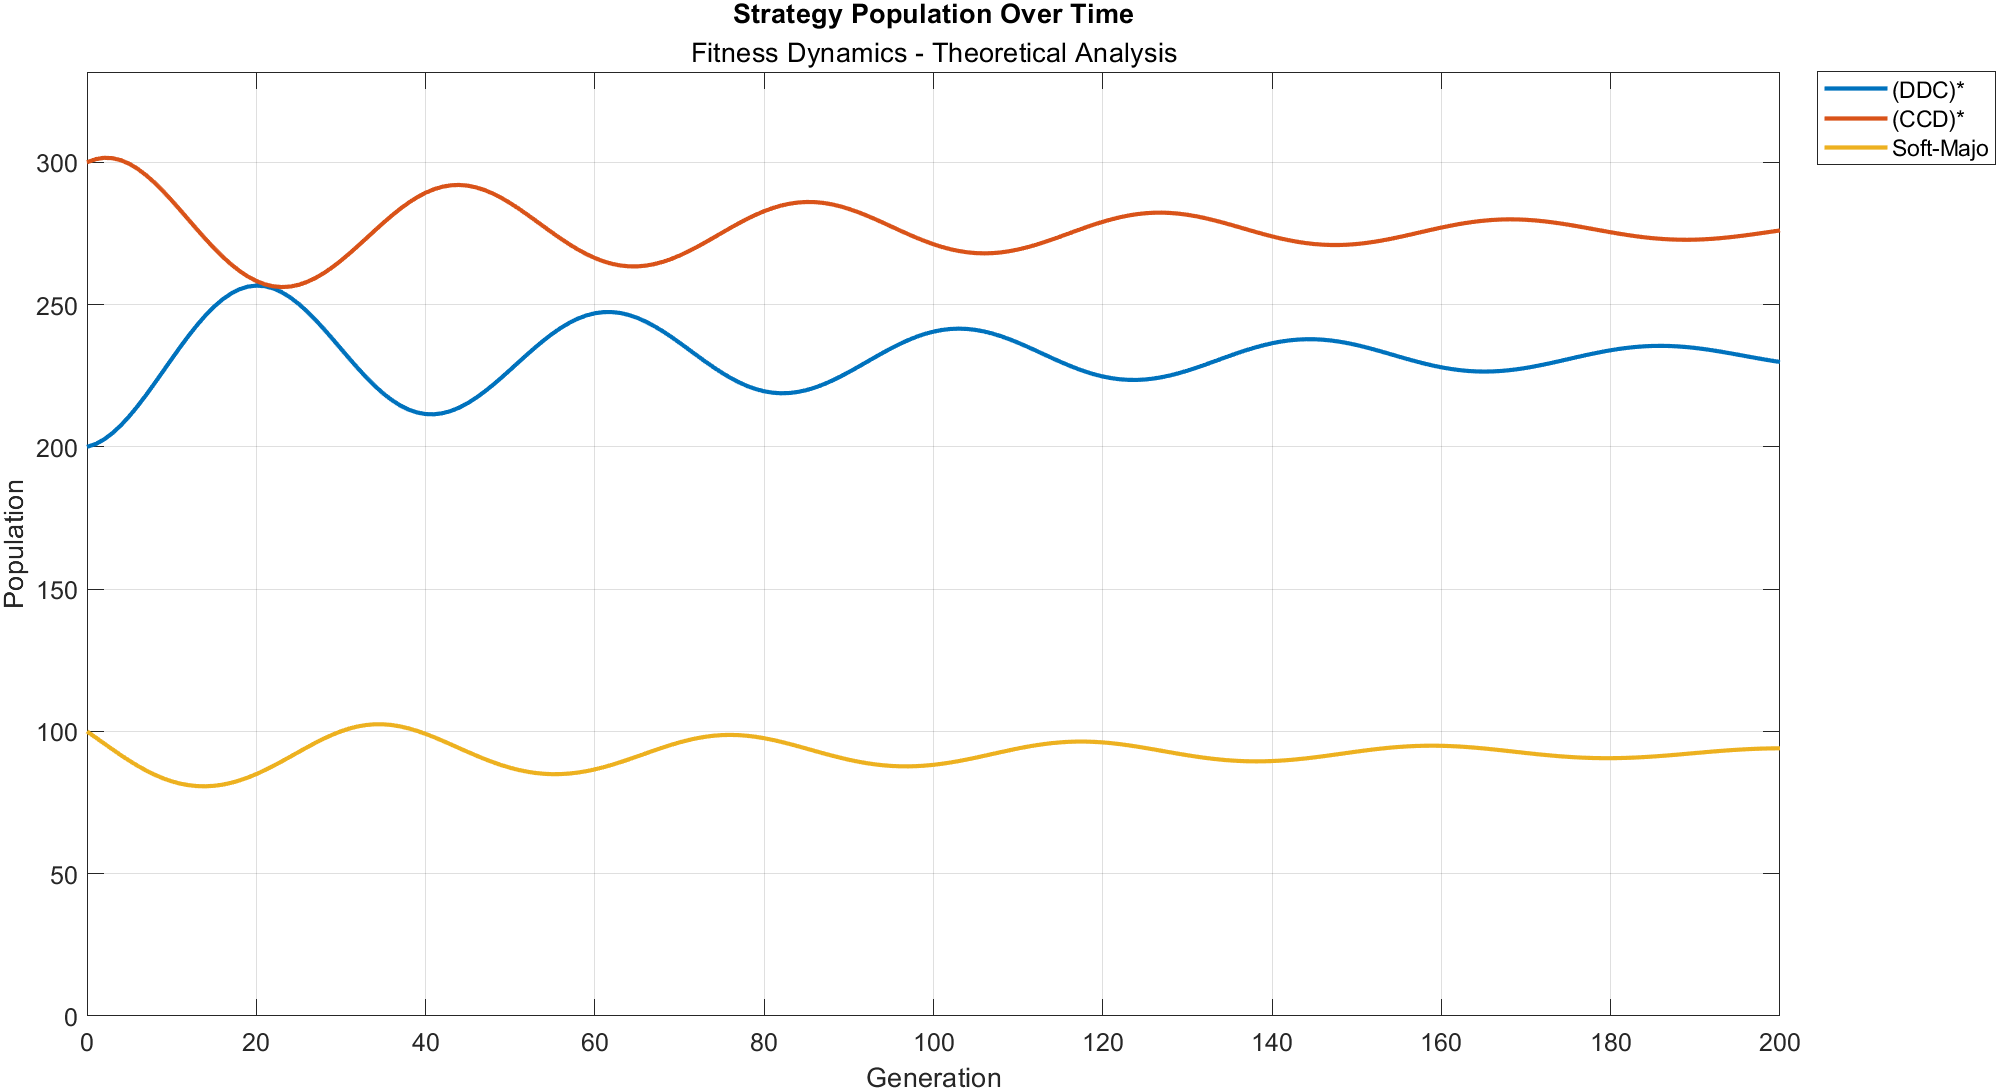
\includegraphics[width=\textwidth]{Graphs/theoretical_fit.png}
    \caption{Θεωρητική ανάλυση με χρήση δεκαδικών παικτών}
    \label{fig:the_fit2_dec}
\end{subfigure}
\hfill
\begin{subfigure}[b]{0.6\textwidth}
    \centering
    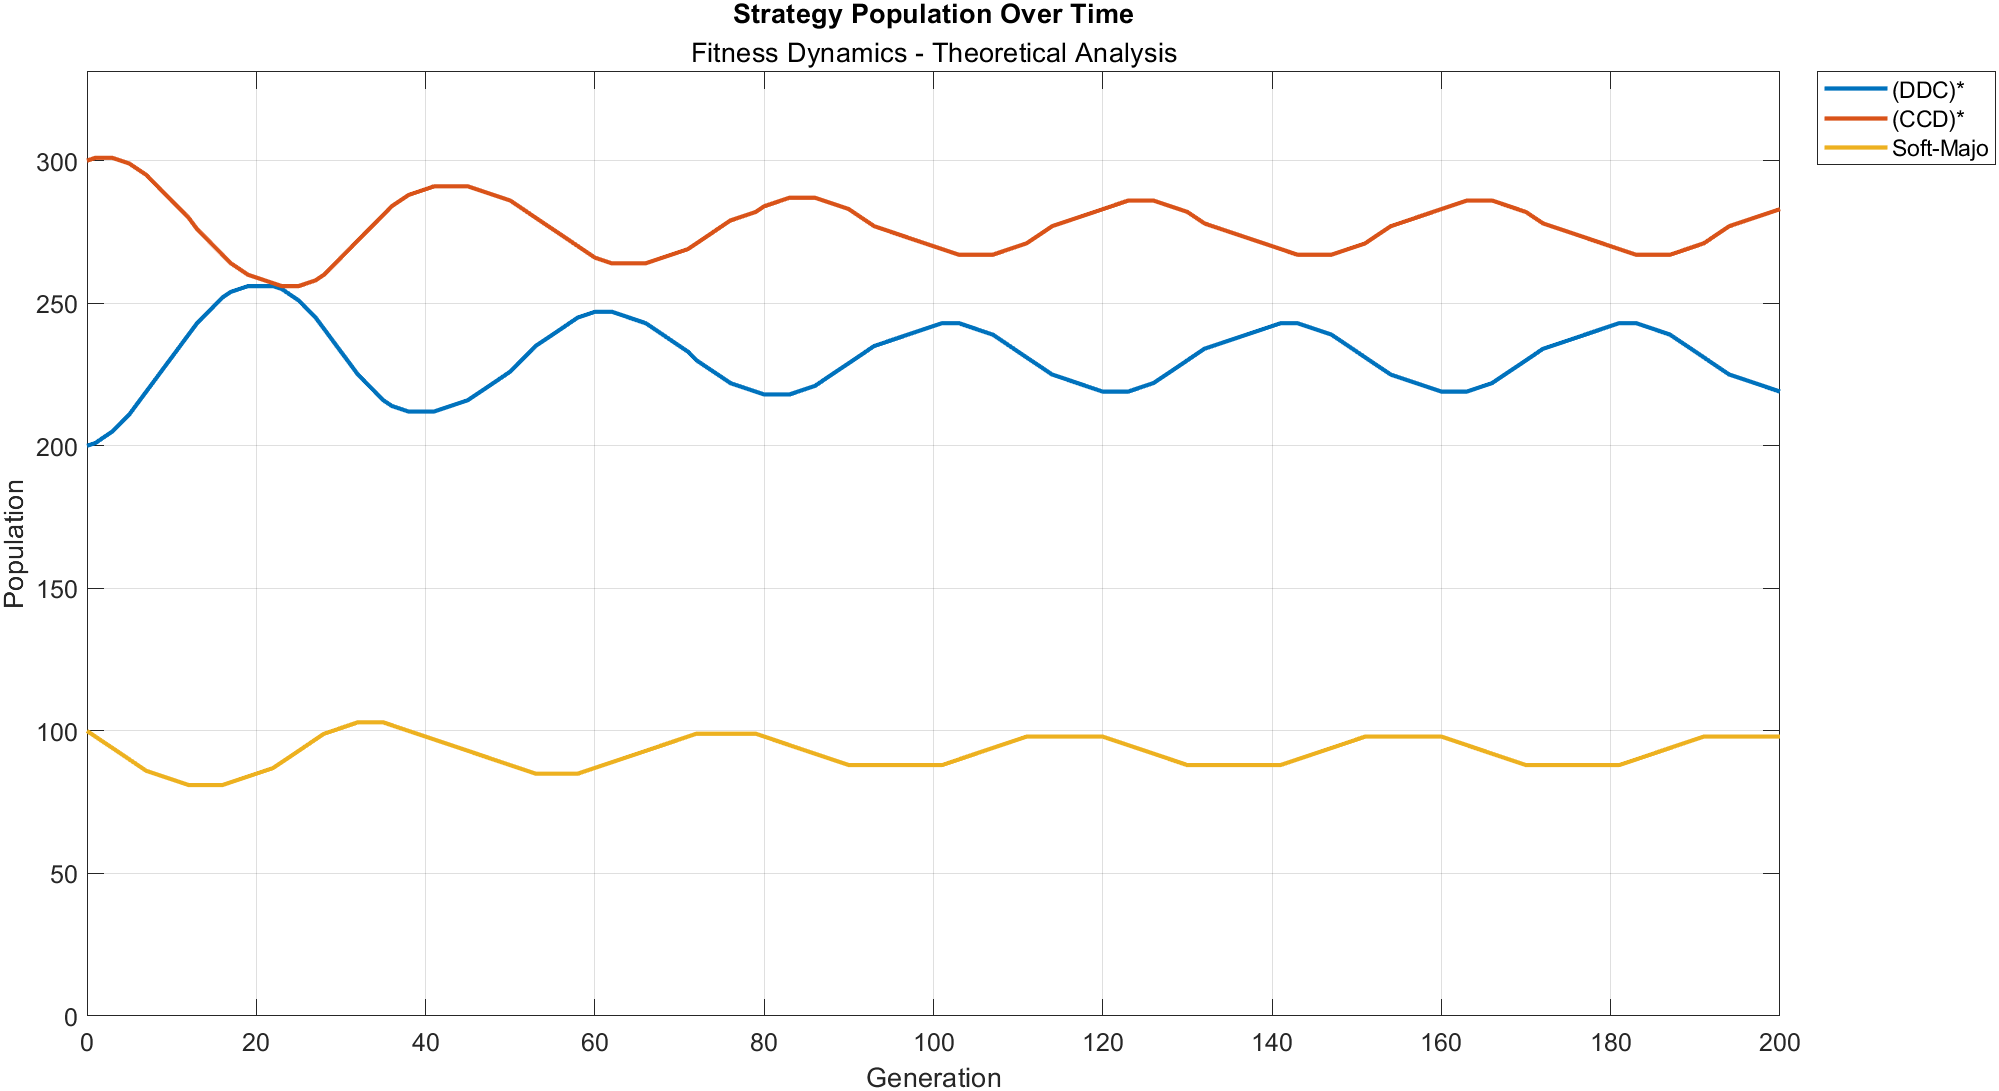
\includegraphics[width=\textwidth]{Graphs/theoretical_fit_pop_red.png}
    \caption{Θεωρητική ανάλυση με αναπροσαρμογή πληθυσμού μέσω της $pop\_redistribute$}
    \label{fig:the_fit2_pr}
\end{subfigure}

\vspace{1em}

% Second row: one centered subfigure
\begin{subfigure}[b]{0.6\textwidth}
    \centering
    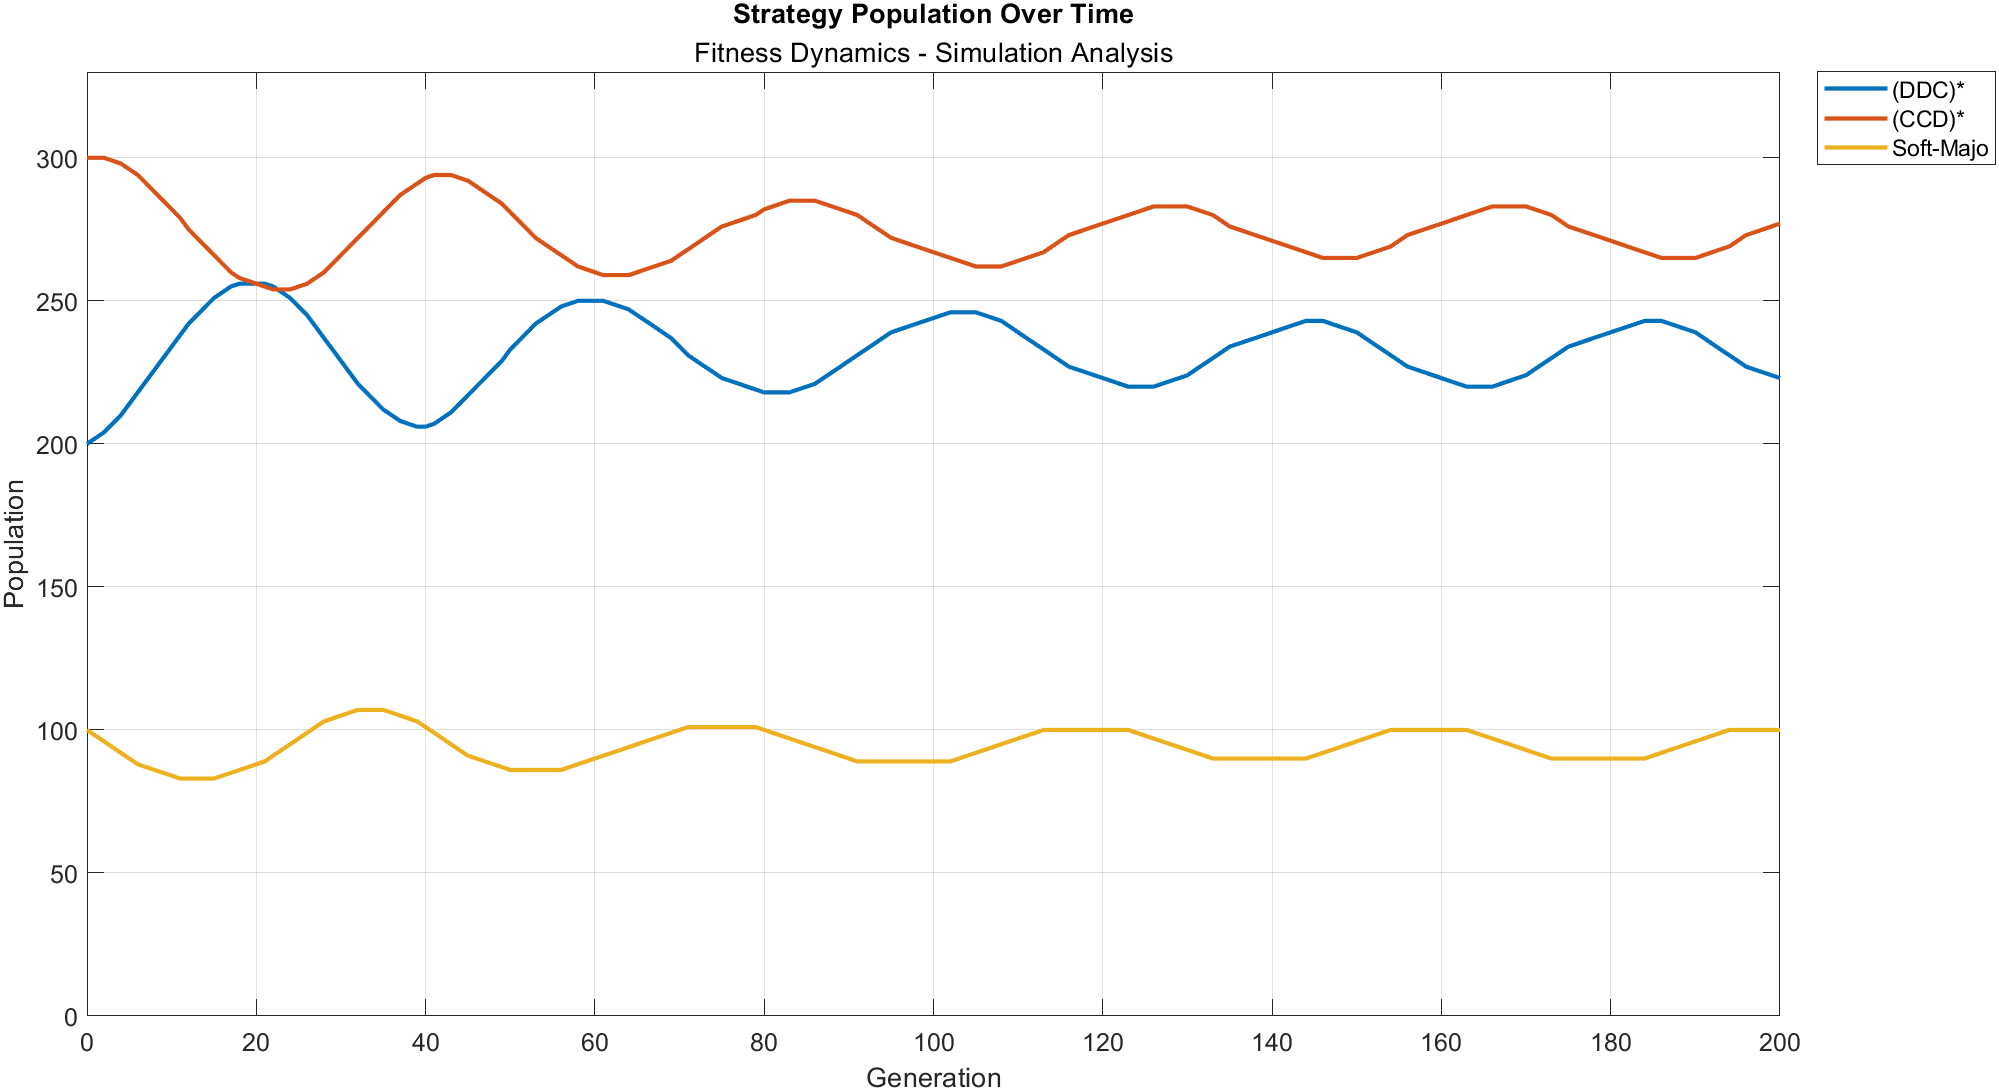
\includegraphics[width=\textwidth]{Graphs/fit_sim2.png}
    \caption{Προσομοίωση με χρήση της $pop\_redistribute$}
    \label{fig:sim_fit2}
\end{subfigure}

\caption{Ανάλυση και προσομοίωση με \foreignlanguage{english}{Fitness Dynamics}}
\end{figure}

\subsubsection*{Εύρεση στρατηγικών και πληθυσμών που δίνουν χάος/απρόβλεπτη συμπεριφορά}
Θα προσπαθήσουμε να βρούμε στρατηγικές και πληθυσμούς αυτών που δίνουν απρόβλεπτες περιοδικές μεταβολές (ο όρος χάος δεν είναι ακριβής, καθώς ενώ οι μεταβολές πληθυσμών είναι αρκετά απρόβλεπτες, εμφανίζουν μια περιοδικότητα).
Μετά από πολλές δοκιμές και προσαρμογές καταλήξαμε σε μια αρχική σύνθεση πληθυσμού \foreignlanguage{english}{All-D: 20, (CD)*: 10, (DDC)*: 10, Soft-Majo: 5, Prober: 30} και τρέχοντας την θεωρητική ανάλυση βρίσκουμε τα αποτελέσματα που φαίνονται στο παρακάτω διάγραμμα (\ref{fig:disordered_os}).
Παρατηρούμε μια κυκλική εναλλαγή κυριαρχίας μεταξύ των στρατηγικών \foreignlanguage{english}{All-D \& (CD)*}, με τις \foreignlanguage{english}{Soft Majo \& Prober} να κερδίζουν περιοδικά πληθυσμό, πριν τον ξαναχάσουν. Παρόλα αυτά η γενική εικόνα του διαγράμματος πληθυσμού δεν θυμίζει κάποια γνωστή συμπεριφορά (αυστηρή μονοτονία, σταθερές ή αποσβεννύμενες ταλαντώσεις).
\begin{figure}[H]
    \centering
    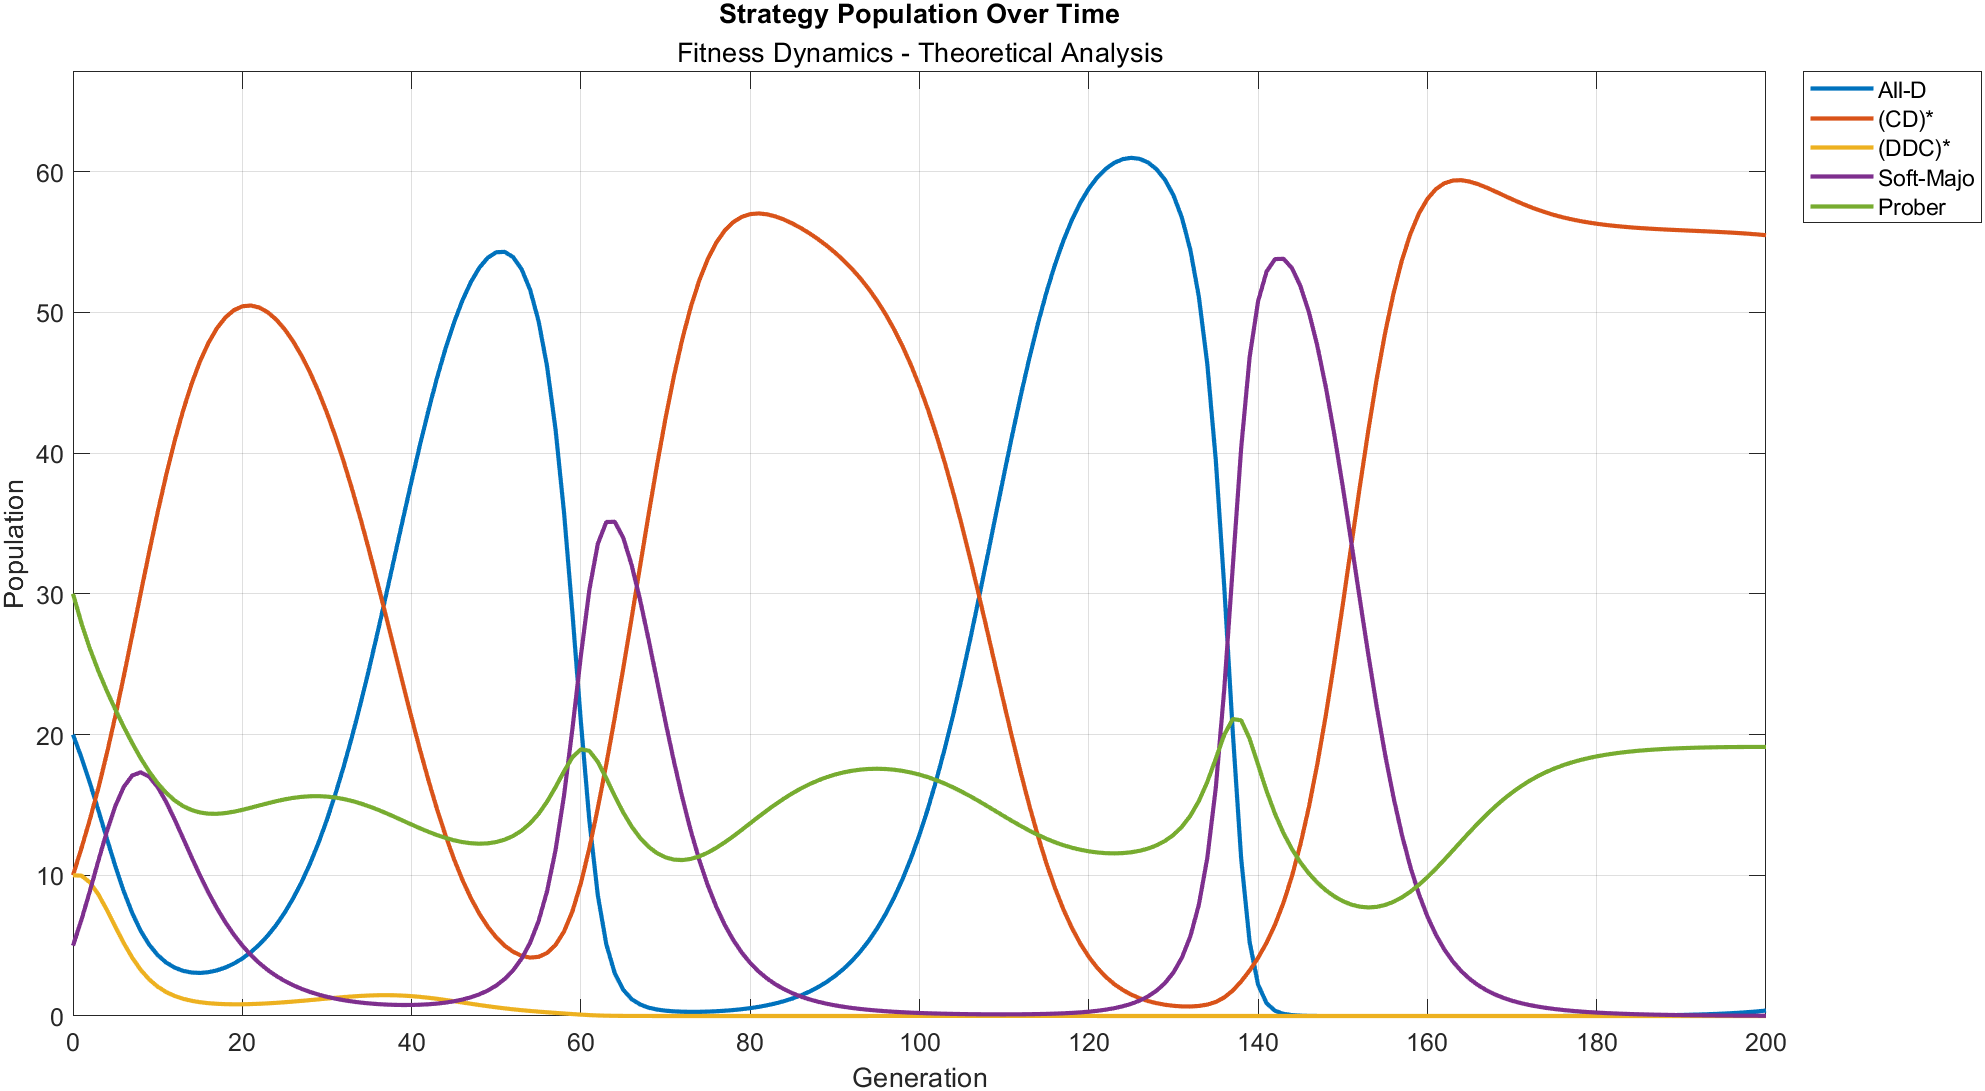
\includegraphics[width=0.8\linewidth]{Graphs/disordered_osc.png}
    \caption{Απρόβλεπτη συμπεριφορά}
    \label{fig:disordered_os}
\end{figure}

\section{Εξελικτικό πρωτάθλημα με \foreignlanguage{english}{Imitation Dynamics}}
\subsection{Προσομοίωση πρωταθλήματος\foreignlanguage{english}{ - TourSimImi}}
Για την προσομοίωση του πρωταθλήματος με χρήση των \foreignlanguage{english}{Imitation Dynamics}, αρχικά υπολογίζουμε τις συνολικές βαθμολογίες των παικτών για κάθε στρατηγική και εντοπίζουμε τις βέλτιστες στρατηγικές βάσει αυτών των βαθμολογιών. Στη συνέχεια, επιλέγονται τυχαία συνολικά $K$ παίκτες από εκείνους που ακολουθούν μη βέλτιστες στρατηγικές, οι οποίοι μεταβάλλουν τη στρατηγική τους υιοθετώντας μία τυχαία από τις βέλτιστες. Τέλος, ανανεώνεται η κατανομή του πληθυσμού των παικτών, λαμβάνοντας υπόψη τις νέες στρατηγικές.

\subsection{Θεωρητική ανάλυση πρωταθλήματος\foreignlanguage{english}{ - TourTheImi}}
Η θεωρητική ανάλυση του πρωταθλήματος με χρήση των \foreignlanguage{english}{Imitation Dynamics} στοχεύει στην εύρεση του πίνακα πιθανοτήτων μετάβασης \(P\) από μία κατάσταση, δηλαδή την κατανομή του πληθυσμού στις στρατηγικές, σε μια άλλη.

\subsubsection*{Υπολογισμός καταστάσεων}
Εάν ορίσουμε \(Ν\) τον συνολικό αριθμό των παικτών του πρωταθλήματος, τότε μπορούμε να υπολογίσουμε όλες τις πιθανές καταστάσεις του πληθυσμού χρησιμοποιώντας την συνάρτηση \foreignlanguage{english}{compositions(N, M)} όπου \(N\) είναι ο συνολικός σταθερός πληθυσμός του πρωταθλήματος, ενώ \(M\) είναι οι ενεργές (με μη μηδενικό πλήθος παικτών) στρατηγικές.
Καταρχάς, μπορούμε απευθείας να θέσουμε την πιθανότητα μιας μετάβασης σε 1, εάν η τρέχουσα κατάσταση έχει μόνο μια στρατηγική με μη μηδενικό αριθμό παικτών (αναγκαστικά θα παραμείνει στην ίδια κατάσταση).
Έπειτα για κάθε πιθανή κατάσταση, υπολογίζουμε το συνολικό σκορ κάθε στρατηγικής, από το οποίο προκύπτουν οι βέλτιστες και μη βέλτιστες στρατηγικές. Επαναπροσδιορίζουμε το \foreignlanguage{english}{K\_actual} (πλήθος \foreignlanguage{english}{imitators}) έτσι ώστε αν έχουμε αρχικά Κ μεγαλύτερο του διαθέσιμου αριθμού παικτών μη βέλτιστων στρατηγικών, να μην βρεθούμε σε αδιέξοδο.
\begin{equation}
\foreignlanguage{english}{K_{actual} = min(K, \text{Total non-best players}})
\end{equation}


\subsubsection*{Υπολογισμός της διαφοράς μεταξύ τρέχουσας κατάστασης - υποψήφιας επόμενης}
Για την τρέχουσα κατάσταση και κάθε υποψήφια επόμενη, φτιάχνουμε το διάνυσμα διαφορών πληθυσμού, $difference\_vector = new\_state - current\_state$ από το οποίο εξάγουμε τα διανύσματα $G$ και $L$, τα οποία μας δείχνουν πόσους παίκτες κέρδισαν οι βέλτιστες στρατηγικές και πόσους έχασαν οι μη βέλτιστες αντίστοιχα. Κάνουμε έναν έλεγχο εγκυρότητας της νέας κατάστασης ελέγχοντας αν το άθροισμα των παικτών στα $G$ και $L$ είναι ίσο με K. Αν η μετάβαση είναι έγκυρη προχωράμε στον υπολογισμό της πιθανότητάς της. Αλλιώς της αναθέτουμε πιθανότητα 0 και προχωράμε στην επόμενη υποψήφια μετάβαση.


\subsubsection*{Υπολογισμός πιθανοτήτων μετάβασης}
Για μια έγκυρη μετάβαση, από μια τρέχουσα κατάσταση σε μια νέα, θέλουμε να υπολογίσουμε την πιθανότητά της. Χωρίζουμε το πρόβλημα σε δύο μέρη.
Αρχικά, υπολογίζουμε την πιθανότητα να επιλέξουμε $K_{actual}$ παίκτες από το σύνολο παικτών των μη βέλτιστων στρατηγικών. Η πιθανότητα αυτή βρίσκεται μέσω της συνάρτησης μάζας πιθανότητας της \textbf{υπεργεωμετρικής κατανομής πολλών μεταβλητών} (αφού έχουμε επιλογή χωρίς επανάληψη).
Έπειτα, υπολογίζουμε την πιθανότητα ανάθεσης αυτών των $K_{actual}$ παικτών στις βέλτιστες στρατηγικές. Η πιθανότητα αυτή βρίσκεται μέσω της συνάρτησης μάζας πιθανότητας της \textbf{πολυωνυμικής κατανομής με ομογενείς πιθανότητες} για κάθε βέλτιστη στρατηγική (ένας \foreignlanguage{english}{imitator} επιλέγει τυχαία και ομοιόμορφα ποια βέλτιστη στρατηγική θα μιμηθεί στην επόμενη γενιά).
Τέλος, συνδυάζουμε τις δύο πιθανότητες με πολλαπλασιασμό για να βρούμε την τελική πιθανότητα μετάβασης. (Η επιλογή και επανάθεση των $K_{actual}$ παικτών είναι ανεξάρτητα γεγονότα)


\subsubsection*{Πίνακας μετάβασης}
Αποθηκεύουμε τον πίνακα μετάβασης μαζί με τις κεφαλίδες για κάθε κατάσταση σε ένα αρχείο \foreignlanguage{english}{Excel} για εύκολη ανάγνωση όταν υπάρχουν πολλές καταστάσεις. 
Ακόμα, αποθηκεύουμε σε ένα άλλο αρχείο \foreignlanguage{english}{Excel} το υπόμνημα των καταστάσεων, δηλαδή τον αριθμό της κατάστασης και την κατανομή του πληθυσμού που αντιπροσωπεύει.
Έχουμε επαληθεύσει πως τα αποτελέσματα είναι ορθά για τιμές $Κ \geq 1$. Για το παράδειγμα $K=1$ με πληθυσμούς \foreignlanguage{english}{(CD)*=1, (DDC)*=2, SOFT-MAJO=1} παραθέτουμε τον πίνακα μετάβασης (Πίνακας \ref{tab:trans_matrix}) μαζί με το υπόμνημα καταστάσεων (Πίνακας \ref{tab:state_matrix}).



\begin{table}[!h]
    \foreignlanguage{english}{
    \centering
    \resizebox{\textwidth}{!}{%
    \begin{tabular}{|l|l|l|l|l|l|l|l|l|l|l|l|l|l|l|l|}
    \hline
        \textbf{Current$\backslash$Next} & \textbf{State 1} & \textbf{State 2} & \textbf{State 3} & \textbf{State 4} & \textbf{State 5} & \textbf{State 6} & \textbf{State 7} & \textbf{State 8} & \textbf{State 9} & \textbf{State 10} & \textbf{State 11} & \textbf{State 12} & \textbf{State 13} & \textbf{State 14} & \textbf{State 15} \\ \hline
        \textbf{State 1} & 1 & 0 & 0 & 0 & 0 & 0 & 0 & 0 & 0 & 0 & 0 & 0 & 0 & 0 & 0 \\ \hline
        \textbf{State 2} & 1 & 0 & 0 & 0 & 0 & 0 & 0 & 0 & 0 & 0 & 0 & 0 & 0 & 0 & 0 \\ \hline
        \textbf{State 3} & 0 & 1 & 0 & 0 & 0 & 0 & 0 & 0 & 0 & 0 & 0 & 0 & 0 & 0 & 0 \\ \hline
        \textbf{State 4} & 0 & 0 & 0 & 0 & 1 & 0 & 0 & 0 & 0 & 0 & 0 & 0 & 0 & 0 & 0 \\ \hline
        \textbf{State 5} & 0 & 0 & 0 & 0 & 1 & 0 & 0 & 0 & 0 & 0 & 0 & 0 & 0 & 0 & 0 \\ \hline
        \textbf{State 6} & 1 & 0 & 0 & 0 & 0 & 0 & 0 & 0 & 0 & 0 & 0 & 0 & 0 & 0 & 0 \\ \hline
        \textbf{State 7} & 0 & 0.5 & 0 & 0 & 0 & 0.5 & 0 & 0 & 0 & 0 & 0 & 0 & 0 & 0 & 0 \\ \hline
        \textbf{State 8} & 0 & 0 & 0 & 0.5 & 0 & 0 & 0 & 0 & 0.5 & 0 & 0 & 0 & 0 & 0 & 0 \\ \hline
        \textbf{State 9} & 0 & 0 & 0 & 0 & 1 & 0 & 0 & 0 & 0 & 0 & 0 & 0 & 0 & 0 & 0 \\ \hline
        \textbf{State 10} & 0 & 0 & 0 & 0 & 0 & 0 & 0 & 0 & 0 & 0 & 0 & 0 & 1 & 0 & 0 \\ \hline
        \textbf{State 11} & 0 & 0 & 0 & 0 & 0 & 0 & 0 & 0 & 0 & 0 & 0 & 0 & 0.5 & 0.5 & 0 \\ \hline
        \textbf{State 12} & 0 & 0 & 0 & 0 & 0 & 0 & 0 & 0 & 1 & 0 & 0 & 0 & 0 & 0 & 0 \\ \hline
        \textbf{State 13} & 0 & 0 & 0 & 0 & 0 & 0 & 0 & 0 & 0 & 0 & 0 & 0 & 0 & 0 & 1 \\ \hline
        \textbf{State 14} & 0 & 0 & 0 & 0 & 0 & 0 & 0 & 0 & 0 & 0 & 0 & 0 & 0 & 0 & 1 \\ \hline
        \textbf{State 15} & 0 & 0 & 0 & 0 & 0 & 0 & 0 & 0 & 0 & 0 & 0 & 0 & 0 & 0 & 1 \\ \hline
    \end{tabular}
    }}
    \caption{\foreignlanguage{greek}{Πίνακας μετάβασης για $K=1$ με πληθυσμούς \foreignlanguage{english}{(CD)*=1, (DDC)*=2, Soft-Majo=1}}}
    \label{tab:trans_matrix}
\end{table}


\begin{table}[!h]
    \foreignlanguage{english}{
    \centering
    \begin{tabular}{|l|l|l|l|}
    \hline
        \textbf{State$\backslash$Strategy} & \textbf{(CD)*} & \textbf{(DDC)*} & \textbf{Soft-Majo} \\ \hline
        \textbf{State 1} & 0 & 0 & 4 \\ \hline
        \textbf{State 2} & 0 & 1 & 3 \\ \hline
        \textbf{State 3} & 0 & 2 & 2 \\ \hline
        \textbf{State 4} & 0 & 3 & 1 \\ \hline
        \textbf{State 5} & 0 & 4 & 0 \\ \hline
        \textbf{State 6} & 1 & 0 & 3 \\ \hline
        \textbf{State 7} & 1 & 1 & 2 \\ \hline
        \textbf{State 8} & 1 & 2 & 1 \\ \hline
        \textbf{State 9} & 1 & 3 & 0 \\ \hline
        \textbf{State 10} & 2 & 0 & 2 \\ \hline
        \textbf{State 11} & 2 & 1 & 1 \\ \hline
        \textbf{State 12} & 2 & 2 & 0 \\ \hline
        \textbf{State 13} & 3 & 0 & 1 \\ \hline
        \textbf{State 14} & 3 & 1 & 0 \\ \hline
        \textbf{State 15} & 4 & 0 & 0 \\ \hline
    \end{tabular}
    }
    \caption{\foreignlanguage{greek}{Πίνακας αντιστοίχισης καταστάσεων-πληθυσμού}}
\label{tab:state_matrix}
\end{table}

\newpage
\subsubsection*{Υπολογισμός τελικού πληθυσμού}
Γνωρίζοντας πλέον τον πίνακα μετάβασης μπορούμε να υπολογίσουμε τον πίνακα πιθανοτήτων για $J$ μεταβάσεις (δηλαδή για $J$ γενιές εξέλιξης). Παίρνουμε $P^{(J)}=P^J$ και βρίσκουμε την αρχική κατάσταση (έστω κατάσταση $i$) βάσει του αρχικού πληθυσμού. Έπειτα, για να βρούμε την αναμενόμενη σύνθεση του πληθυσμού μετά από $J$ γενιές πηγαίνουμε στην $i$-οστή σειρά του πίνακα $P^J$ και παίρνουμε το άθροισμα των πληθυσμών κάθε κατάστασης, επί την πιθανότητα αυτής της κατάστασης, για αρχική κατάσταση $i$.

\subsection{Πειράματα}
\subsubsection*{Πρωτάθλημα μεταξύ των στρατηγικών \foreignlanguage{english}{(CD)*, (DDC)*, Soft-Majo}}
Πραγματοποιούμε το ίδιο πρωτάθλημα που υλοποιήσαμε στο πρώτο πειράμα με \foreignlanguage{english}{Fitness Dynamics} αλλά τώρα με χρήση των \foreignlanguage{english}{Imitation Dynamics}. Θεωρούμε ότι τρεις παίκτες μιμούνται την καλύτερη στρατηγική σε κάθε γενεά (Κ=3). Τα αποτελέσματα της θεωρητικής ανάλυσης αλλά και της προσομοίωσης παρουσιάζονται στα σχήματα \ref{fig:imi_the1} και \ref{fig:imi_sim1} αντίστοιχα. Υπενθυμίζουμε ότι για εξοικονόμηση χρόνου στην προσομοίωση έχουμε θεωρήσει Τ=100 γύρους ανά παιχνίδι και 80 γενιές, ενώ για την θεωρητική ανάλυση λόγω της εκθετικής απαίτησης σε μνήμη, αρχικοποιήσαμε τον πληθυσμό της κάθε στρατηγικής σε 9 παίκτες αντί για 100 που είναι στην προσομοίωση.

Παρατηρούμε ότι οι πληθυσμοί των στρατηγικών μειώνονται γραμμικά αφού σε κάθε γενιά η/οι βέλτιστη/ες στρατηγική/ές κερδίζουν ένα σταθερό αριθμό παικτών τον οποίον αντίστοιχα χάνουν οι μη βέλτιστες στρατηγικές. Συνεπώς το πρωτάθλημα συγκλίνει γρήγορα σε μια κατάσταση όπου επιβιώνει μόνο η βέλτιστη στρατηγική.
Τόσο στην θεωρητική ανάλυση όσο και στην προσομοίωση μετά από ικανό αριθμό γενεών, η στρατηγική \foreignlanguage{english}{(CD)*} αναδεικνύεται ως η επικρατέστερη.

\begin{figure}[h]
\centering

\begin{subfigure}[b]{0.9\textwidth}
    \centering
    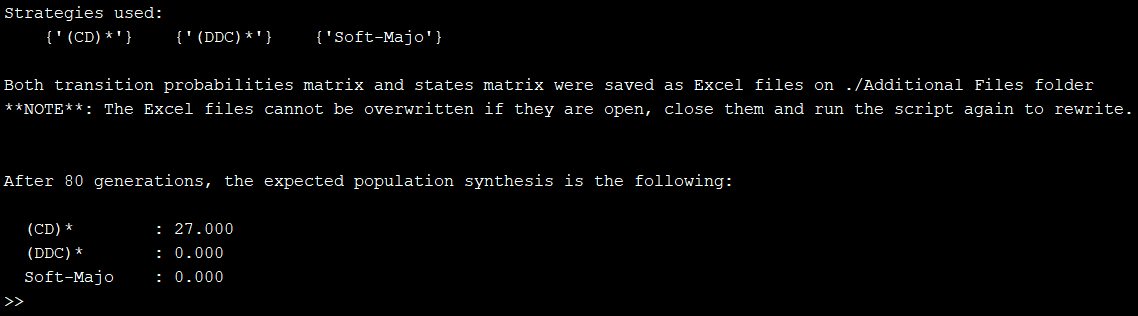
\includegraphics[width=\textwidth]{Graphs/imi_the1.png}
    \caption{Θεωρητική ανάλυση - Συνολικοί παίκτες 9}
    \label{fig:imi_the1}
\end{subfigure}
\hfill
\vspace{1em}
\begin{subfigure}[b]{0.9\textwidth}
    \centering
    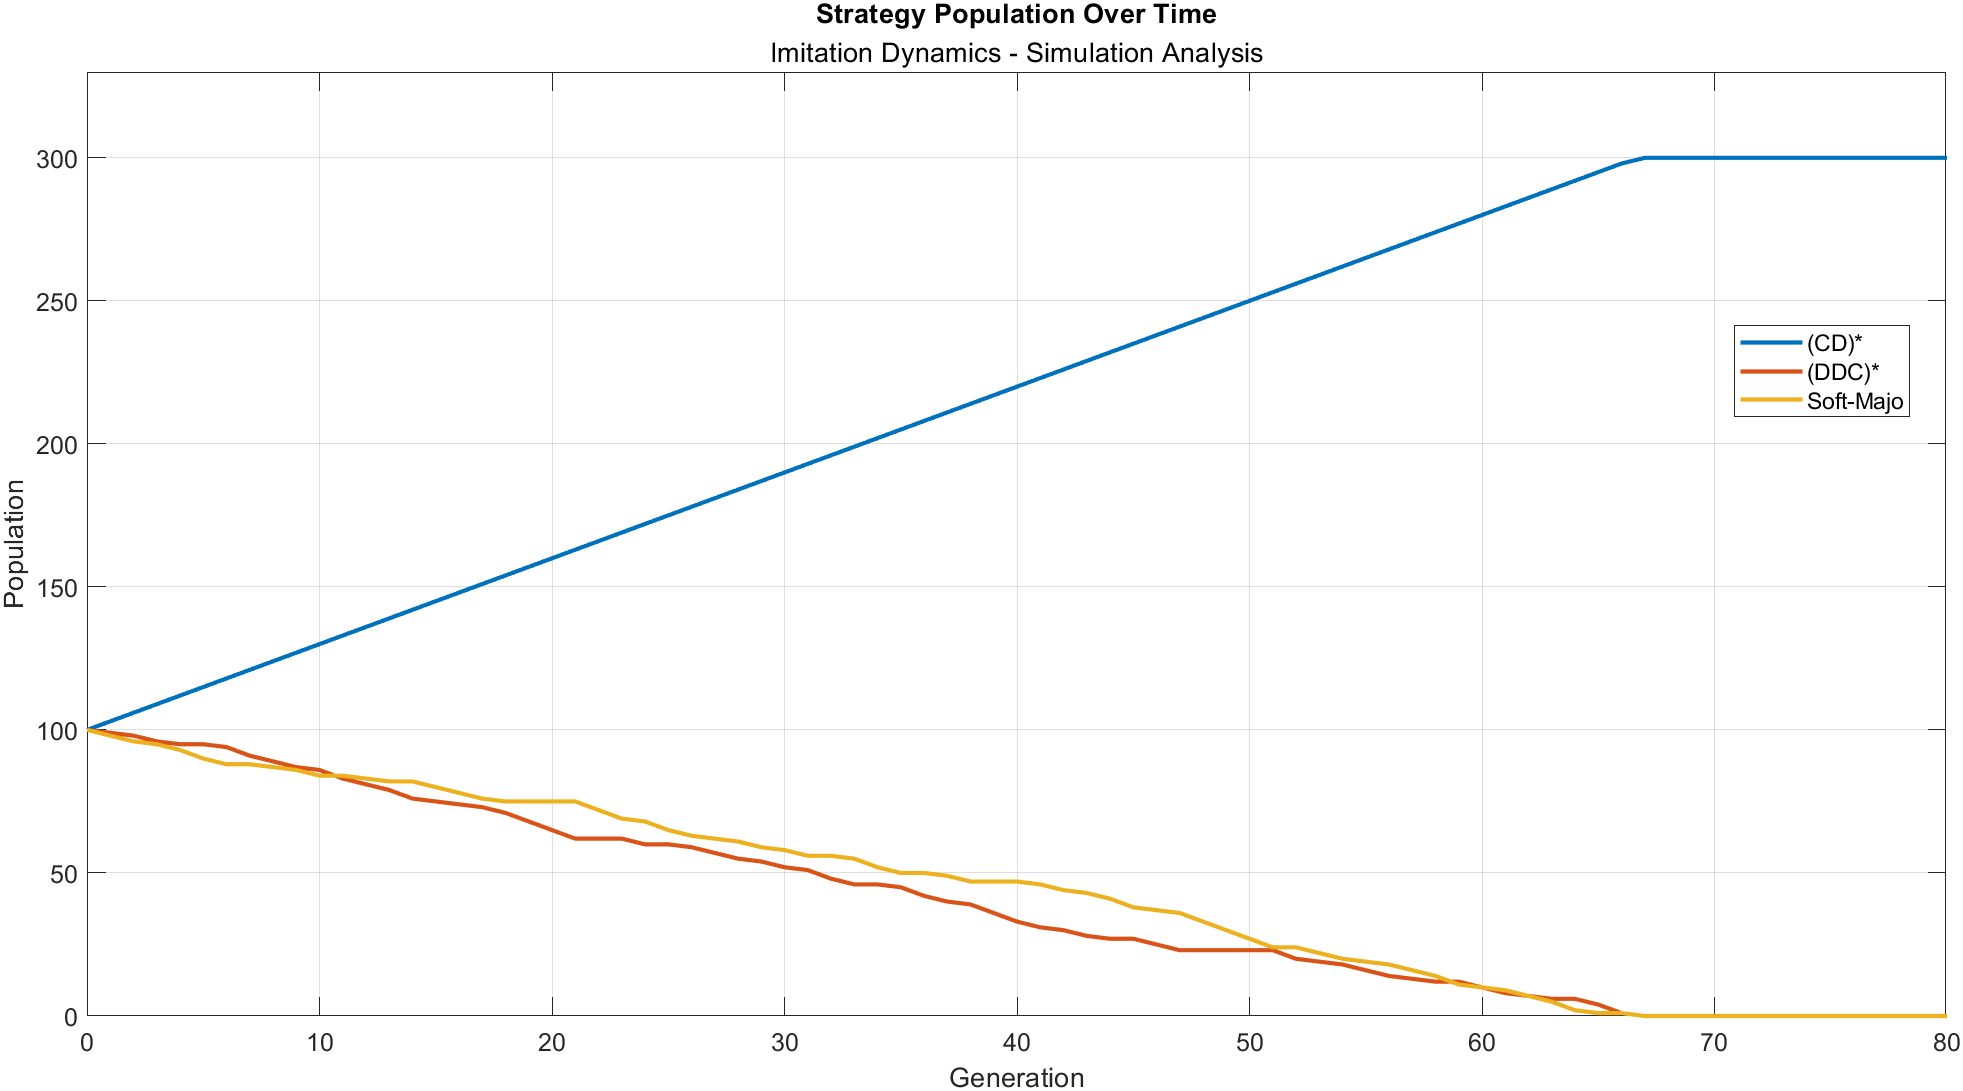
\includegraphics[width=\textwidth]{Graphs/imi_sim1.png}
    \caption{Προσομοίωση - Συνολικοί παίκτες 100}
    \label{fig:imi_sim1}
\end{subfigure}
\caption{Θεωρητική ανάλυση και προσομοίωση με παίκτες} \foreignlanguage{english}{(CD)*, (DDC)*, (S-M)}
\end{figure}


\subsubsection*{Πρωτάθλημα μεταξύ των στρατηγικών \foreignlanguage{english}{(CCD)*, (DDC)*, Soft-Majo}}

Πραγματοποιούμε το ίδιο πρωτάθλημα που υλοποιήσαμε στο δεύτερο πειράμα με \foreignlanguage{english}{Fitness Dynamics} αλλά τώρα με χρήση των \foreignlanguage{english}{Imitation Dynamics}. Θεωρούμε ότι τρεις παίκτες μιμούνται την καλύτερη στρατηγική σε κάθε γενεά (Κ=3). Τα αποτελέσματα της θεωρητικής ανάλυσης αλλά και της προσομοίωσης παρουσιάζονται στα σχήματα \ref{fig:imi_the2} και \ref{fig:imi_sim2} αντίστοιχα. Χρειάζεται να σημειωθεί ότι για εξοικονόμηση χρόνου στην προσομοίωση έχουμε θεωρήσει Τ=100 γύρους ανά παιχνίδι και 80 γενιές, ενώ για την θεωρητική ανάλυση λόγω της εκθετικής απαίτησης σε μνήμη, αρχικοποιήσαμε τον πληθυσμό της κάθε στρατηγικής σε 6, 9 και 3 παίκτες (για να ικανοποιήσουμε την απαίτηση $N\leq9$ διατηρώντας την αναλογία) αντί για 200, 300 και 100 αντίστοιχα, που είναι στην προσομοίωση.
Παρατηρούμε και πάλι μια γραμμική μεταβολή του πληθυσμού κάθε στρατηγικής ενώ έπειτα από ικανό αριθμό γενεών, τόσο στην θεωρητική ανάλυση όσο και στην προσομοίωση, επικρατεί η στρατηγική \foreignlanguage{english}{(CCD)*}.

\begin{figure}[H]
\centering
\begin{subfigure}[b]{0.9\textwidth}
    \centering
    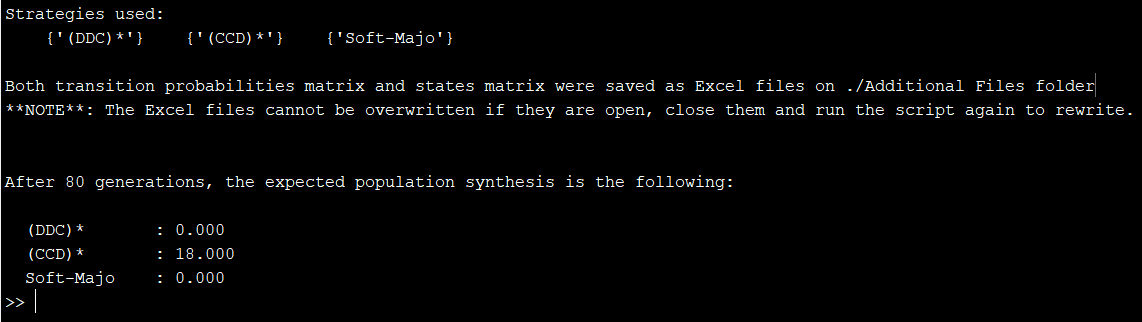
\includegraphics[width=\textwidth]{Graphs/imi_the2.png}
    \caption{Θεωρητική ανάλυση - \foreignlanguage{english}{(CCD)*=9, (DDC)*=6, (S-M)=3} παίκτες}
    \label{fig:imi_the2}
\end{subfigure}
\hfill
\vspace{1em}
\begin{subfigure}[b]{0.9\textwidth}
    \centering
    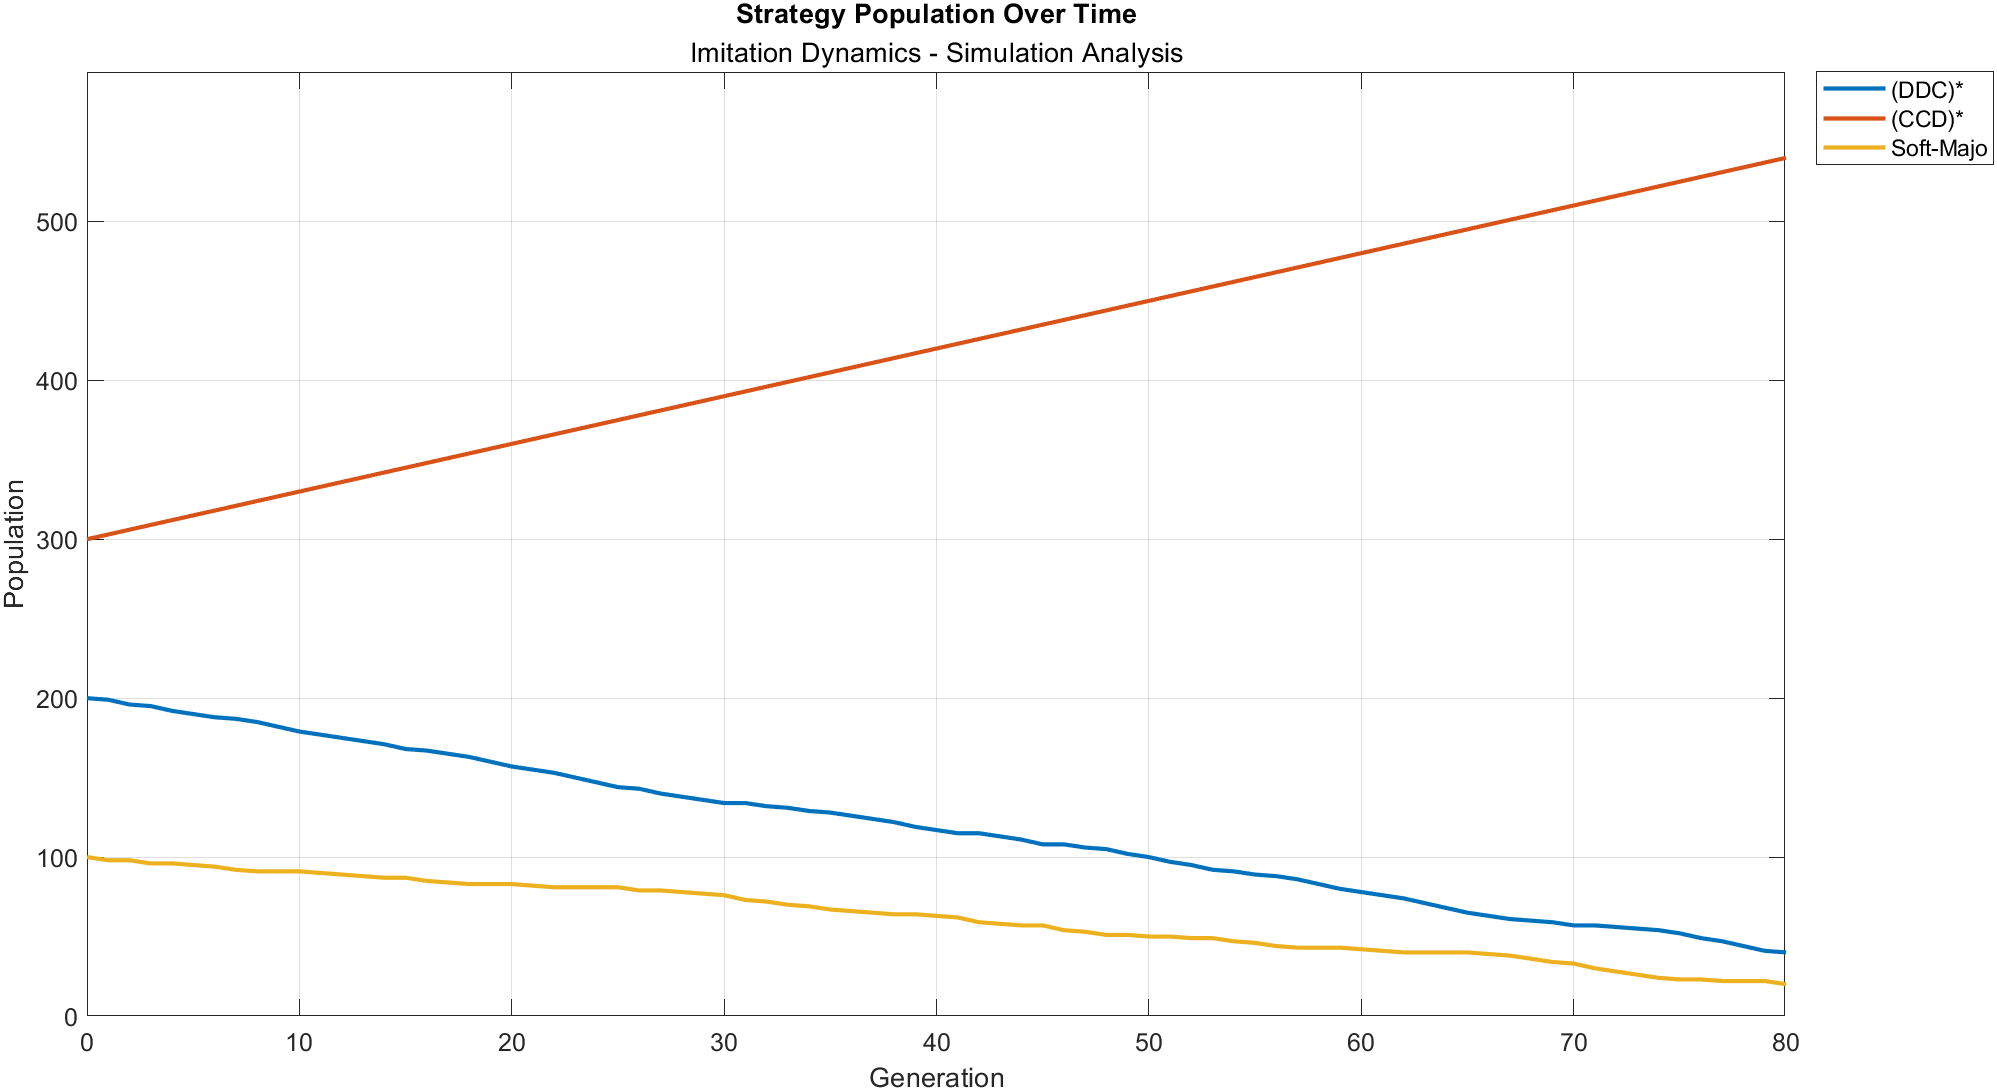
\includegraphics[width=\textwidth]{Graphs/imi_sim2.png}
    \caption{Προσομοίωση - \foreignlanguage{english}{(CCD)*=300, (DDC)*=200, (S-M) = 100} παίκτες}
    \label{fig:imi_sim2}
\end{subfigure}
\caption{Θεωρητική ανάλυση και προσομοίωση με παίκτες} \foreignlanguage{english}{(CCD)*, (DDC)*, (S-M)}
\end{figure}



\newpage
\section{Σύγκριση μεθόδων}
Παρατηρούμε ότι υπάρχουν σημαντικές διαφορές μεταξύ των δύο τεχνικών αναδιανομής του πληθυσμού μεταξύ γενεών. Η αναδιανομή μέσω \foreignlanguage{english}{Fitness Dynamics} μπορεί παρουσιάσει ταλαντώσεις ή και χάος στην σύνθεση πληθυσμών των στρατηγικών, ενώ μπορεί να απαιτηθεί μεγάλος αριθμός γενεών έως ότου αναδειχθούν σταθερές τάσεις ή μέχρι να φτάσουμε σε σύγκλιση. Ειδικότερα, εάν το πρώτο πείραμα διεξαγόταν μόνο για 20 γενιές, το τελικό αποτέλεσμα θα διέφερε σημαντικά σε σχέση με αυτό που θα είχαμε για 50 γενιές.

Αντιθέτως, η αναδιανομή μέσω \foreignlanguage{english}{Imitation Dynamics} φαίνεται πως οδηγεί σε μονότονες και γραμμικές μεταβολές πληθυσμού, καθώς εκ φύσεως ενισχύει τις ισχυρές στρατηγικές και εξασθενεί τις αδύναμες, πάντα κατά τον σταθερό παράγοντα Κ.

Ουσιαστικά η διαφορά των δύο δυναμικών έγκειται στο γεγονός πως στην \foreignlanguage{english}{Fitness Dynamics} το κέρδος μιας βέλτιστης στρατηγικής σε σχέση με μια μη βέλτιστη είναι ανάλογο της διαφοράς της ισχύος τους (είναι σχετικό). Δηλαδή όσο πιο ισχυρή είναι μια στρατηγική σε σχέση με τις υπόλοιπες τόσο περισσότερο θα ενισχυθεί.
Αυτή η παρατήρηση εξηγεί και τις συχνά απρόβλεπτες συμπεριφορές στην σύνθεση των πληθυσμών.
Αντίθετα στην \foreignlanguage{english}{Imitation Dynamics} δεν έχει σημασία η σχετική, αλλά η απόλυτη διαφορά ισχύος, μεταξύ βέλτιστων και μη-βέλτιστων στρατηγικών. Μια βέλτιστη στρατηγική θα ενισχυθεί το ίδιο (κατά Κ) ανεξάρτητα του πόσο καλύτερη είναι από τις μη-βέλτιστες.
Αυτή η παρατήρηση εξηγεί και την μονοτονική μεταβολή των πληθυσμών.

\end{document}


